\documentclass[xcolor={table, dvipsnames}]{beamer}
\usepackage[utf8]{inputenc}

\usepackage{utopia} %font utopia imported
\usetheme{Madrid}
\usecolortheme{default}
\usepackage{listings}

\usepackage{hyperref}
\hypersetup{
    colorlinks=true,
    linkcolor=blue,
    filecolor=magenta,      
    urlcolor=cyan,
}

\urlstyle{same}

\newcommand\boldblue[1]{\textcolor{blue}{\textbf{#1}}}

%------------------------------------------------
%Information to be included in the title page:
\title{Computer Architecture}

\subtitle{What computer contains and how it works}

\author{Nguyen The Minh}
\institute{Electronics and Computer Science Home}
\date{Computing Conference, Oct 2050}

%\logo{
\includegraphics[height=1.5cm]{atom.png}}

%End of title page
%-------------------------------------------------

%------------------------------------------------------------
%The next block of commands puts the table of contents at the 
%beginning of each section and highlights the current section:

\AtBeginSection[]
{
  \begin{frame}
    \frametitle{Table of Contents}
    \tableofcontents[currentsection]
  \end{frame}
}
%------------------------------------------------------------

\begin{document}

\frame{\titlepage}

%---------------------------------------------------------
%This block of code is for the table of contents after
%the title page
\begin{frame}
\frametitle{Table of Contents}
\tableofcontents
\end{frame}
%---------------------------------------------------------

\section{Computer History}
\begin{frame}
\frametitle{Pre-20th Century}

\begin{columns}
\column{0.5\textwidth}
\begin{figure}[h!]
  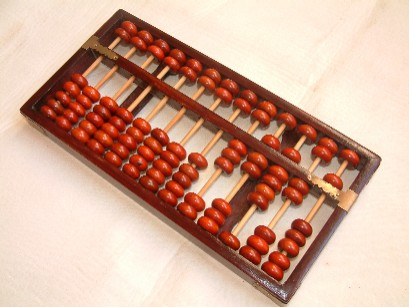
\includegraphics[height=2.5cm]{img/abacus.jpeg}
    \caption{A Chinese Abacus, 2nd BC}
\end{figure}
\column{0.5\textwidth}
\begin{figure}[h!]
  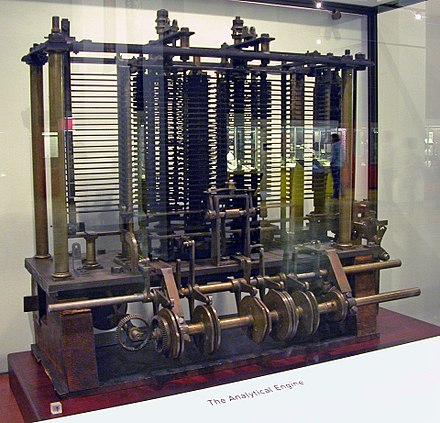
\includegraphics[height=2.5cm]{img/AnalyticalMachine.jpg}
    \caption{1833, Analytical Engine, London Museum}
\end{figure}
\end{columns}

\end{frame}

\begin{frame}
\frametitle{Advent of Digital Computer}

\textbf{Kurt Gödel's} 1931, \textit{Incompleteness Theorem}: universal arithmetic-based formal language \newline \pause

\textbf{Alan Turing} 1936, \textit{On Computable Numbers}:  formal and simple hypothetical devices - Turing Machine  \newline \pause

\textbf{Von Neumann} 1947, \textit{Von Neumann Architecture}: stored-program computers \newline \pause

\textbf{Manchester Baby} 1948, \textit{First stored-program computer} 

\end{frame}

\begin{frame}
\frametitle{First digital computer}

\begin{columns}
\column{0.5\textwidth}
\begin{figure}[h!]
  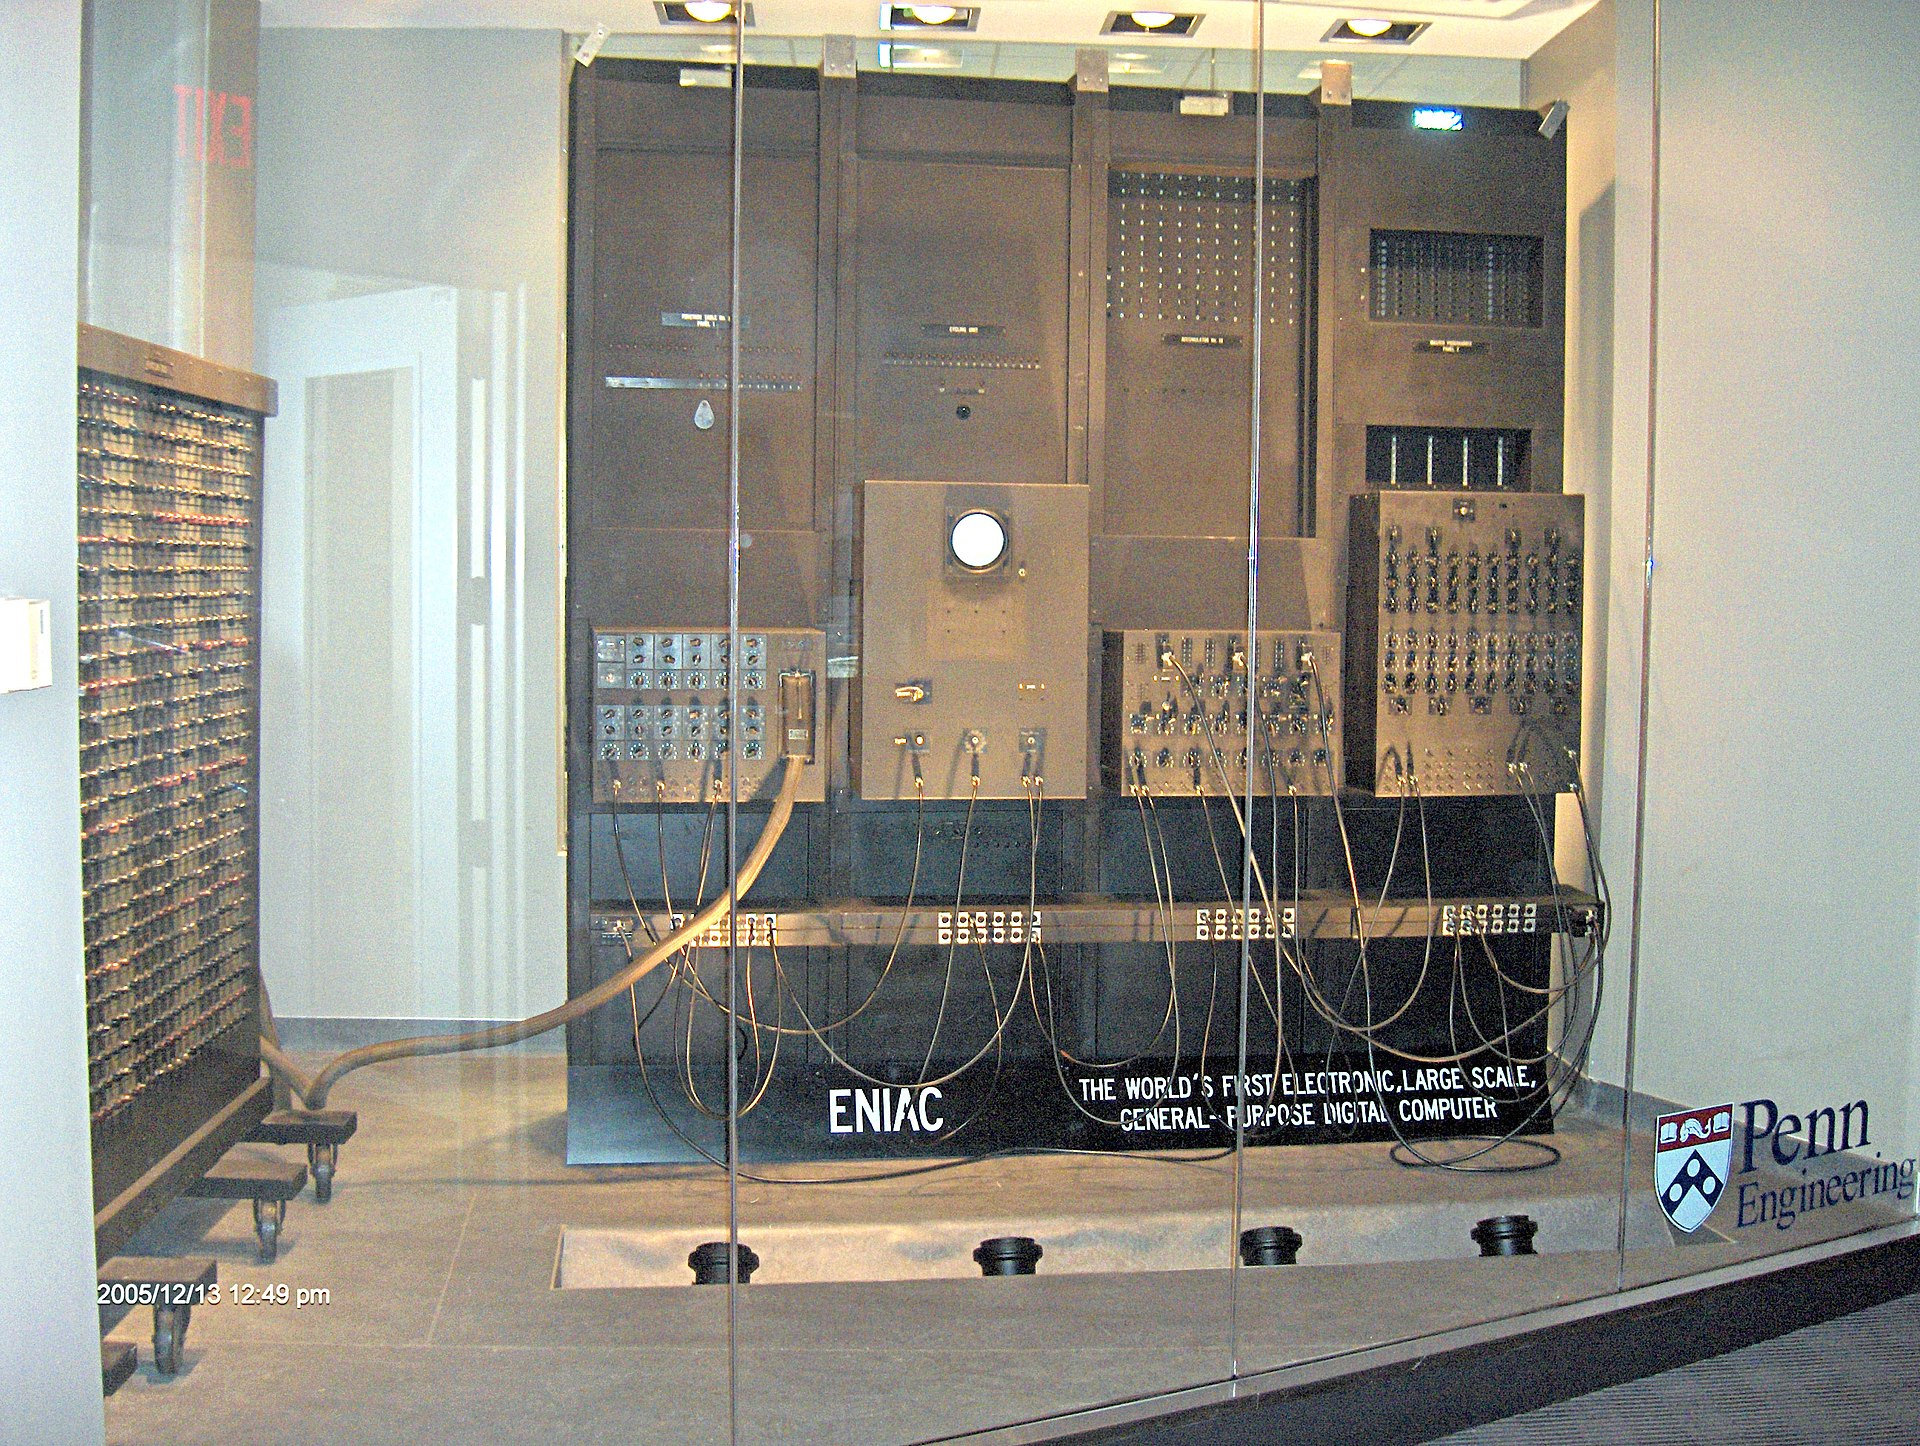
\includegraphics[height=2.5cm]{img/ENIAC.jpg}
    \caption{ENIAC - first electronic computer - 1945}
\end{figure}
\column{0.5\textwidth}
\begin{figure}[h!]
  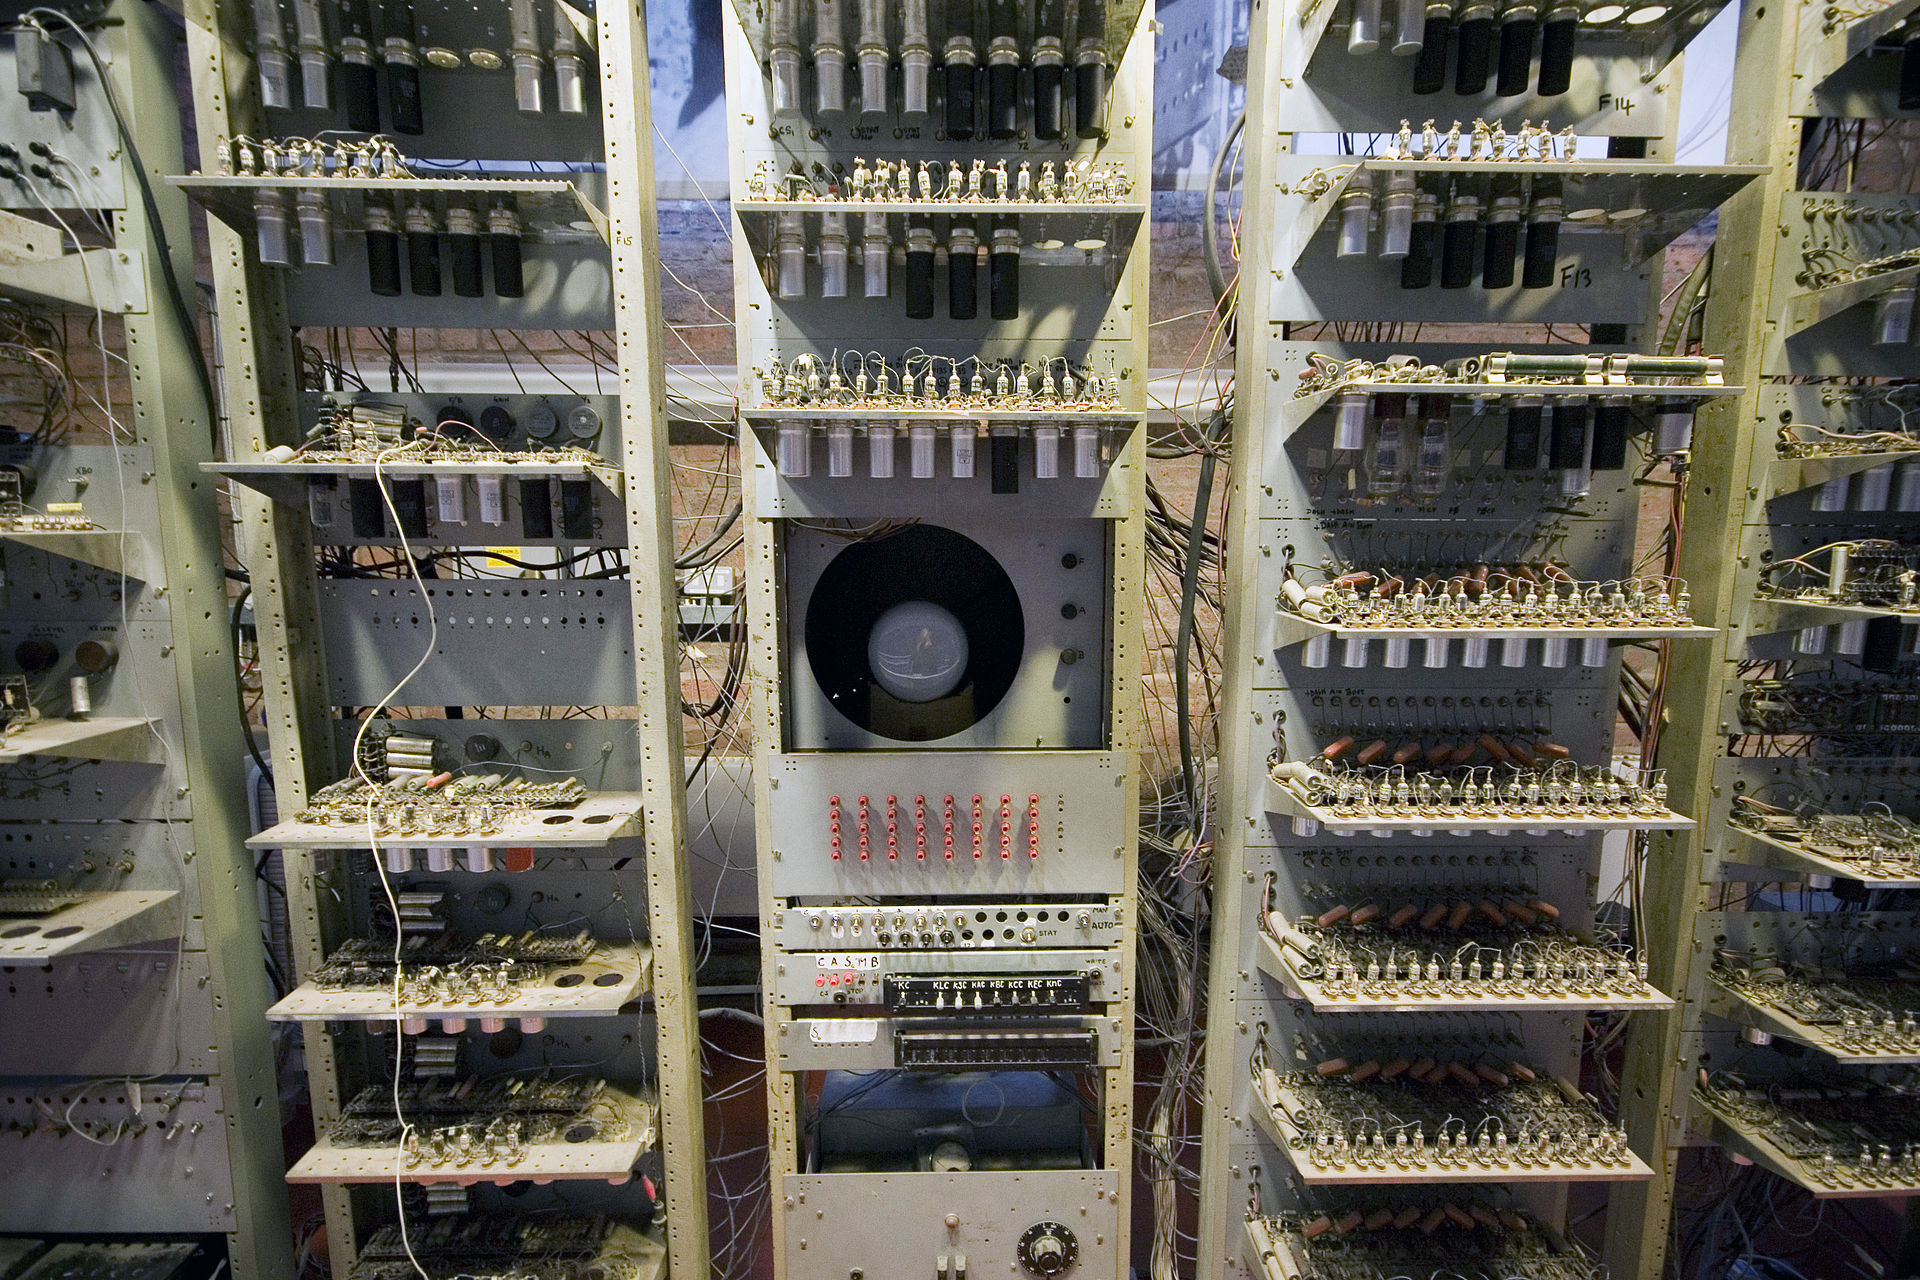
\includegraphics[height=2.5cm]{img/manchester_baby.jpg}
    \caption{Manchester Baby, 1948}
\end{figure}
\end{columns}

\end{frame}

\begin{frame}
\frametitle{Simiconductor Industry}

\begin{figure}[h!]
  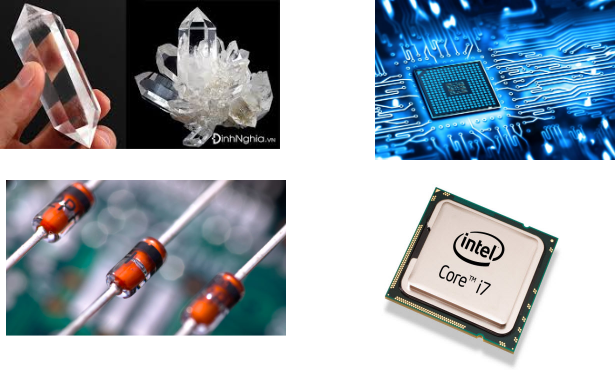
\includegraphics[height=4cm]{img/computer_architecture-simiconductor.png}
    \caption{Silicon Valley}
\end{figure}

Transistor, CMOS, IC

 RAM, ROM

LSIC, Microprocessor,

\href{https://en.wikipedia.org/wiki/History_of_computing_hardware_(1960s\%E2\%80\%93present)}{Wikipedia - Computer Hardware History}
 
\end{frame}

\section{Computer Organization}

\begin{frame}
\frametitle{Modern Digital Computer}
\begin{figure}[h!]
  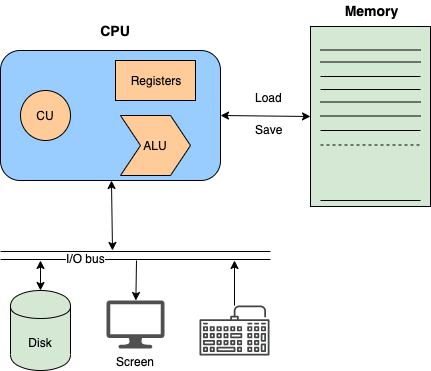
\includegraphics[height=6cm]{img/computer_organization.png}
    \caption{Modern computer organization}
\end{figure}
\end{frame}

\begin{frame}
\frametitle{Building Material}
\begin{figure}[h!]
  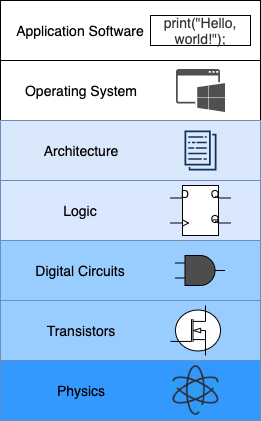
\includegraphics[height=6cm]{img/digital_abstraction.png}
    \caption{Digital Abstraction Layers}
\end{figure}
\end{frame}

\begin{frame}
\frametitle{Logic Circuits}
\begin{columns}
\column{0.25\textwidth}
\begin{figure}[h!]
  \includegraphics[height=2cm]{img/CMOS_inverter.png}
\end{figure}
\column{0.75\textwidth}
\begin{figure}[h!]
  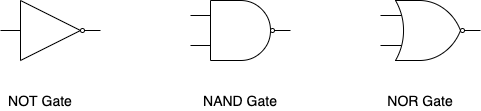
\includegraphics[height=2cm]{img/basic_gates.png}
\end{figure}
\end{columns}
\end{frame}

\begin{frame}
\frametitle{Complex Logic Circuits}
\begin{columns}
\column{0.5\textwidth}
\begin{figure}[h!]
  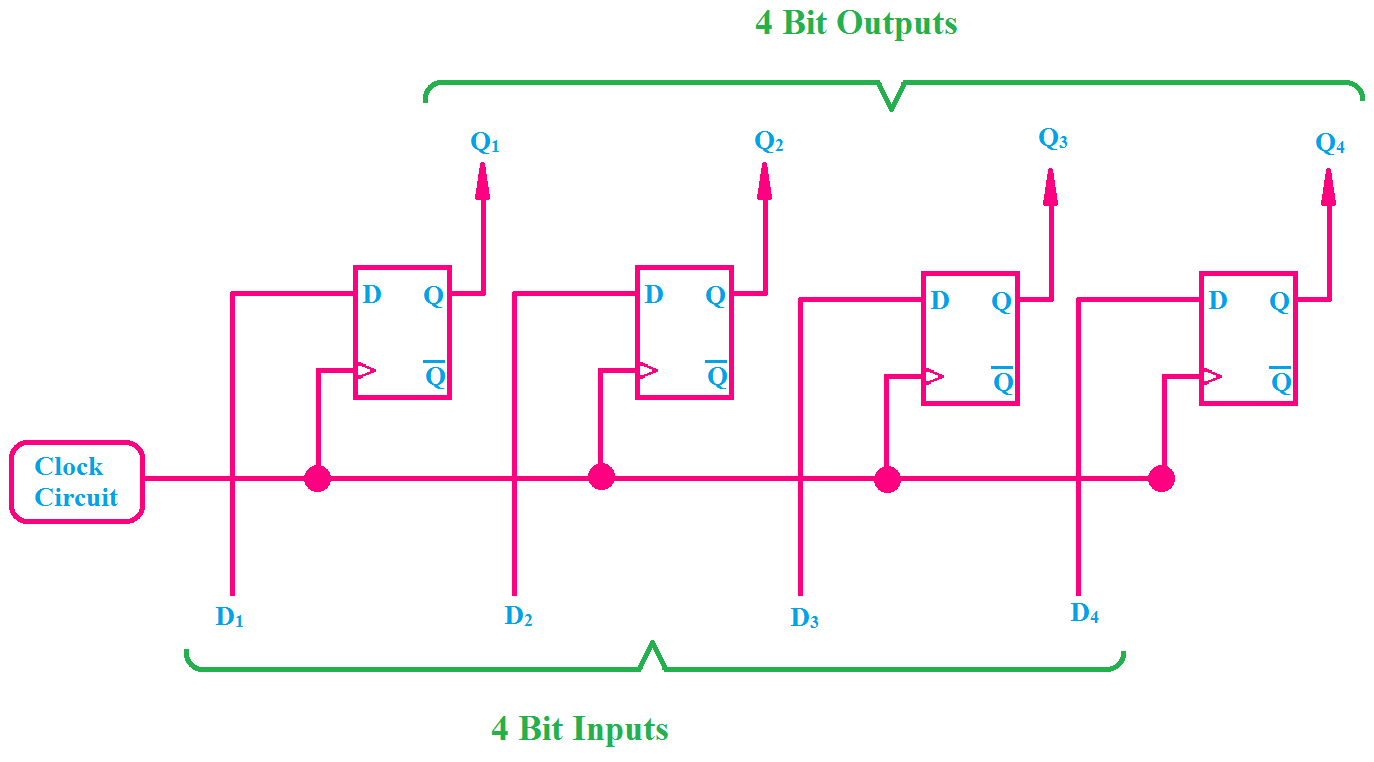
\includegraphics[height=3cm]{img/register.png}
\end{figure}
\column{0.5\textwidth}
\begin{figure}[h!]
  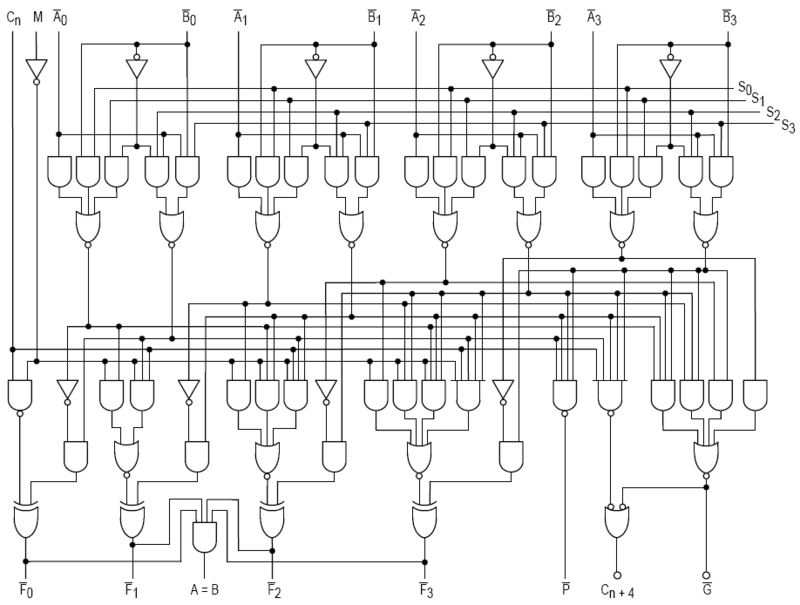
\includegraphics[height=3cm]{img/alu.png}
\end{figure}
\end{columns}
\end{frame}

\section{Instruction Set}

\begin{frame}
\frametitle{How CPU work?}
\begin{figure}[h!]
  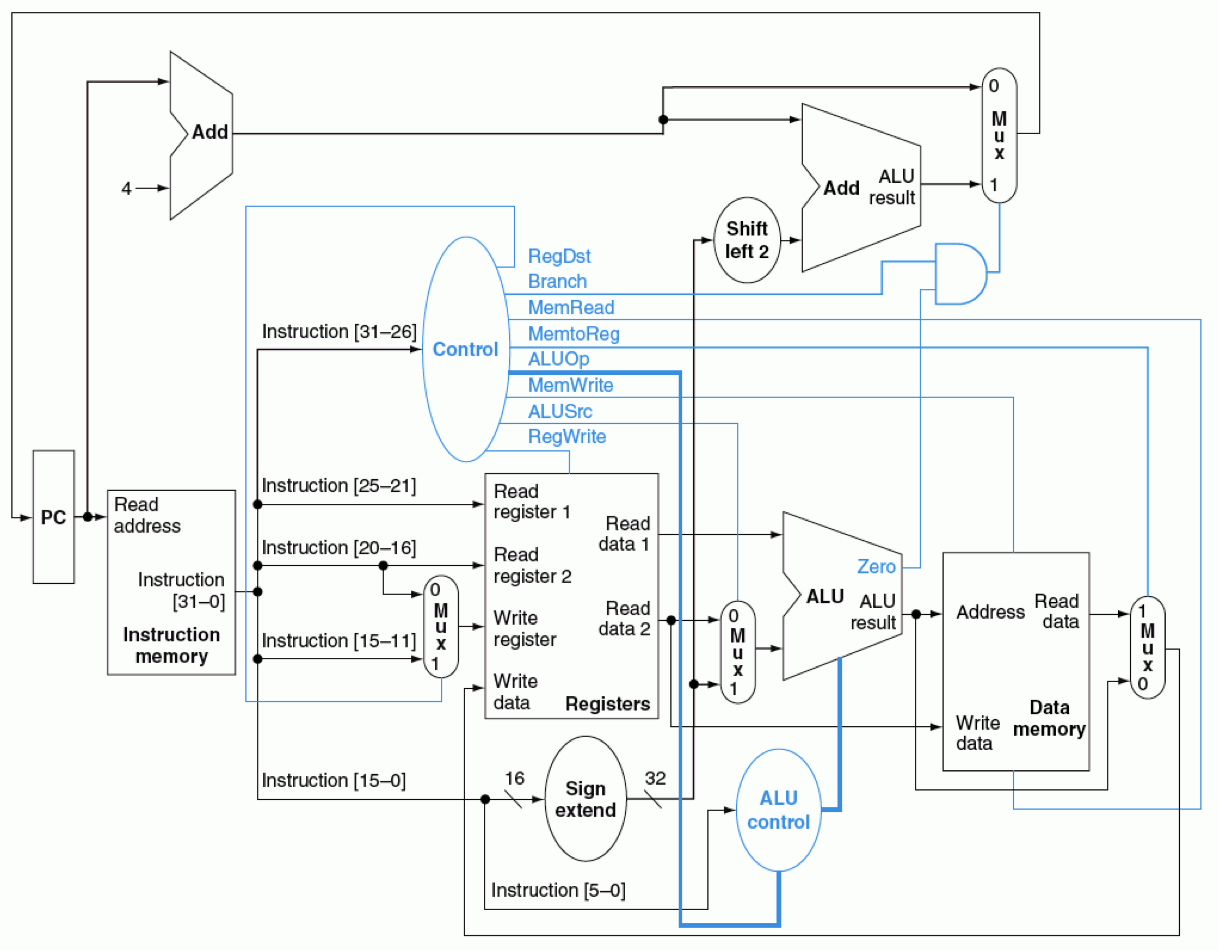
\includegraphics[height=6cm]{img/single_cycle_datapath.png}
\end{figure}

\end{frame}

\begin{frame}
\frametitle{Instructions}

\begin{table}[h!]
\centering
 \begin{tabular}{| c c |} 
\hline
 \boldblue{High-Level Code}  & \boldblue{Assembly Code}   \\ 
 a = b + c & add a, b, c \\ 
 a = b - c & sub a, b, c \\ 
 \hline
\end{tabular}
\caption{Computer Instructions} \pause
\end{table}

\begin{table}[h!]
 \begin{tabular}{| c c |} 
\hline
 \boldblue{High-Level Code}  & \boldblue{Assembly Code}   \\ 
 a = b + c - d & add t, b, c \\ 
   & sub a, t, d \\ 
 \hline
\end{tabular}
\caption{Complex Instructions} 
\end{table}
\end{frame}

\begin{frame}
\frametitle{Operands: Registers, Memory, and Constants}
Instruction operates on \texttt{operands} \newline \pause

Operands stored in registers or memory \newline \pause

Or be constants stored in the instruction itself \newline \pause

Memory is large, but slow
\end{frame}

\begin{frame}
\frametitle{Registers}
\begin{table}[h!]
\centering
{\rowcolors{2}{SkyBlue}{white}
\begin{tabular}{ |p{3cm}| c |p{5cm}|  }
\hline
\rowcolor{NavyBlue}
\textcolor{white}{Name} & \textcolor{white}{Number} & \textcolor{white}{Use}  \\
\hline
\$0 & 0 & the constant value 0 \\
\$at & 1   & assembler temporary \\
\$v0-\$v1 & 2-3 & function return value \\
\$a0-\$a3    & 4-7 & function arguments \\
\$t0-\$t7 & 8-15 & temporary variables \\
\$s0-\$s7 & 16-23 & saved variables   \\
\$t8-\$t9 & 24-25 & temporary variables \\
\$k0-\$k1 & 26-27 & OS temporaries \\
\$gp & 28 & global pointer \\
\$sp & 29 & stack pointer \\
\$fp & 30 & frame pointer \\
\$ra & 31 & function return address \\
\hline
\end{tabular}
}
\caption{MIPS register set}
\end{table}
 \end{frame}
 
 \begin{frame}
 \frametitle{High-Level Code to Assembly}
 Assume \texttt{a-c} held in registers \texttt{\$s0-\$s2} and \texttt{f-j} are in \texttt{\$s3-\$s7} \newline
 
 \begin{example}
 a = b - c;
 
 f = (g + h) - (i + j);
 \end{example}
  
 \end{frame}
 
 \begin{frame}
 \frametitle{Memory}
 \begin{figure}
 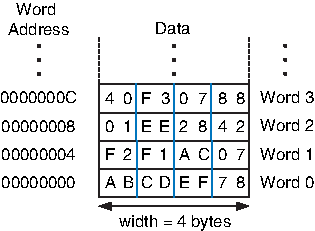
\includegraphics{img/byte-address-memory.pdf}
 \caption{Byte-addressable memory}
 \end{figure}
 \end{frame}

 \begin{frame}
 \frametitle{Memory Access}
 \begin{example}
\$s3, 1(\$0) \# read memory word 1 into \$s3
\newline

\$s7, 5(\$0) \# write \$s7 to memory word 5
 \end{example}
 \end{frame}
 
 \begin{frame}
 \frametitle{Constans/Immediates}
 \begin{table}[h!]
\centering
 \begin{tabular}{| c p{6cm} |} 
\hline
 \boldblue{High-Level Code}  & \boldblue{Assembly Code}   \\ 
 a = a + 4 & addi \$0, \$0, 4 \# \$0 = a, \$s1 = b \\ 
 a = a - 12 & addi \$0, \$0, -12 \\
 \hline
\end{tabular}
\caption{Immediate Operands}
\end{table}
 \end{frame}
 
 \begin{frame}
 \frametitle{Machine Language}
 Digital circuits understand only 1’s and 0’s \newline
 
 Fixed-length instruction: all instructions are encoded with 32 bits \newline
 \begin{itemize}
 \item
R-Type \textit{register-type}
\item
I-Type \textit{immediate-type}
\item
J-Type \textit{jump-type}
\end{itemize}  
 \end{frame}
 
\begin{frame}
\frametitle{R-Type Instructions}
 \begin{figure}
 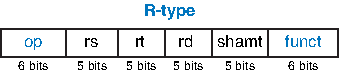
\includegraphics{img/r-type-instruction.pdf}
 \caption{R-Type Format}
 \end{figure}
  \begin{figure}
 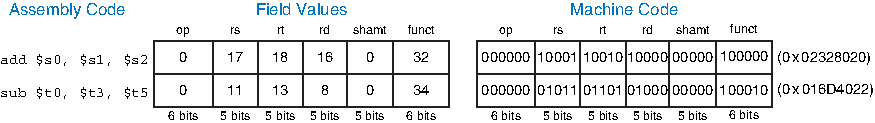
\includegraphics[scale=0.8]{img/r-type-machine-code.pdf}
 \caption{R-Type machine code}
 \end{figure}
\end{frame}

\begin{frame}
\frametitle{I-Type Instructions}
 \begin{figure}
 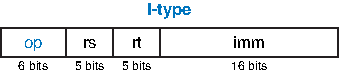
\includegraphics{img/i-type-instruction.pdf}
 \caption{I-type instruction format}
 \end{figure}
   \begin{figure}
 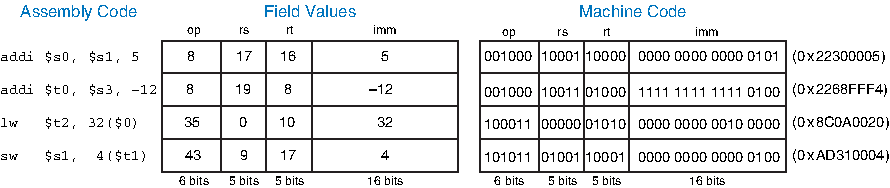
\includegraphics[scale=0.8]{img/i-type-machine-code.pdf}
 \caption{I-type machine code}
 \end{figure}
\end{frame}

\begin{frame}
\frametitle{J-Type Instructions}
 \begin{figure}
 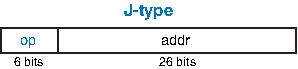
\includegraphics{img/j-type-instruction.pdf}
 \caption{J-type instruction format}
 \end{figure}
 \begin{figure}
 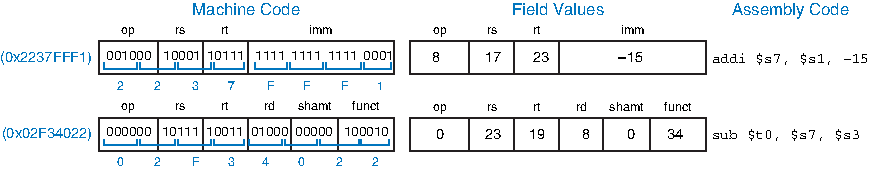
\includegraphics[scale=0.8]{img/machine-to-assembly.pdf}
 \caption{Machine code to assembly}
 \end{figure}
\end{frame}

\begin{frame}
\frametitle{Stored  Program}
\begin{figure}
 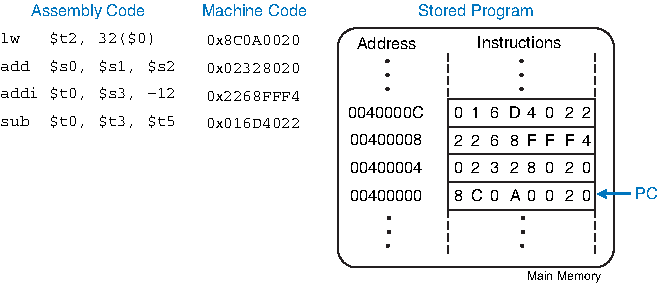
\includegraphics{img/stored-program.pdf}
 \caption{Stored program in memory}
 \end{figure}
\end{frame}

\section{Programming}

\begin{frame}
\frametitle{Arithmetic/Logical Instructions}
\begin{figure}
 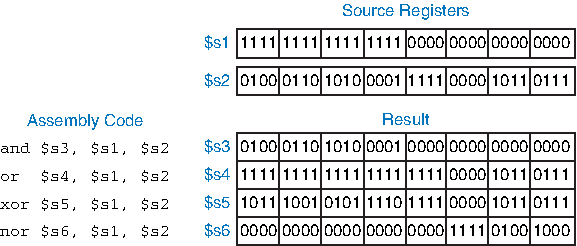
\includegraphics{img/logical-instructions.pdf}
 \caption{Logical instructions}
 \end{figure}
\end{frame}

\begin{frame}[fragile]
\frametitle{Branch}
branch if equal (beq) and branch if not equal (bne)

\begin{lstlisting}[ basicstyle=\ttfamily]
addi $s0,$0,4 #$s0=0+4=4
addi $s1,$0,1 #$s1=0+1=1
sll $s1, $s1, 2 #$s1 = 1 << 2 = 4
beq $s0, $s1, target #$s0 == $s1, so branch
sub $s1, $s1, $s0  #not executed 
target:
add $s1, $s1, $s0  
\end{lstlisting}
\end{frame}

\begin{frame}[fragile]
\frametitle{Jump}
  \begin{lstlisting}[language=C,  basicstyle=\ttfamily,keywordstyle=\color{blue}]     
int sum = 0;
for (i = 0; i != 10; i = i + 1) { 
 sum = sum + i ;
}
   \end{lstlisting} \pause

  \begin{lstlisting}[basicstyle=\ttfamily]     
# $s0 = i, $s1 = sum
 add $s1, $0, $0	    
 addi $s0,$0,0
 addi $t0, $0, 10
 
for:
 beq $s0, $t0, done
 add $s1, $s1, $s0
 addi $s0, $s0, 1
 j for
 
done:
   \end{lstlisting}
\end{frame}

\begin{frame}[fragile]
\frametitle{Function Calls}
\begin{columns}
\column{0.5\textwidth}
 \begin{lstlisting}[language=C,  basicstyle=\ttfamily,keywordstyle=\color{blue}]     
int main() {
 int y;
 y = sum(2, 3);
 ...
}
   \end{lstlisting}
 \column{0.5\textwidth}
 \begin{lstlisting}[language=C,  basicstyle=\ttfamily,keywordstyle=\color{blue}]     
int sum(int x, int y) {
  return x + y;
}
   \end{lstlisting}
\end{columns} \pause

\begin{columns}
\column{0.5\textwidth}
 \begin{lstlisting}[basicstyle=\ttfamily,keywordstyle=\color{blue}]     
# $s0 = y
main:
 addi $a0, $s0, 2
 addi $a1, $s0, 3
 jal sum
 add $s0, $v0, $0
   \end{lstlisting}
 \column{0.5\textwidth}
 \begin{lstlisting}[basicstyle=\ttfamily,keywordstyle=\color{blue}]     
# $s0 = result
sum:
 add $v0, $a0, $a1
 jr $ra
   \end{lstlisting}
\end{columns}
\end{frame}

\begin{frame}
\frametitle{Futher ...}
\begin{itemize}
\item Data allocation
\item Memory Hierarchy and Caches
\item I/O System
\item Processor Design
\item Digital Circuits
\end{itemize}
\end{frame}
\end{document}